\documentclass[a4paper,11pt]{article}
\usepackage[T1]{fontenc}
\usepackage[utf8]{inputenc}
\usepackage{lmodern}
\usepackage{graphicx}
\usepackage{float} 
\usepackage[francais]{babel}
\usepackage{setspace}

\onehalfspacing


\title{\LARGE{Projet composants distribués}\\\bigskip \textbf{Morse Translator}}
\author{Guillaume LAROYENNE\\
   Informatique et réseau,\\
   ENSISA,\\
   2A\\
   \bigskip
   \texttt{guillaume.laroyenne@uha.fr}
   }
\date{\today}

\begin{document}

  \maketitle
      
  \newpage

	\section{Présentation}
	\subsection{Description}
	Vous voulez envoyer des messages en code morse mais vous ne le connaissez pas le langage ? Alors le composant "Morse Translator" est fait pour vous. Ce composant vous permettra de traduire vos textes en morse d'un simple clic. Il vous permettra également de visualiser et d'écouter votre message.
	
    \subsection{Aperçu}
    \begin{figure}[H]
    	\begin{center}
    		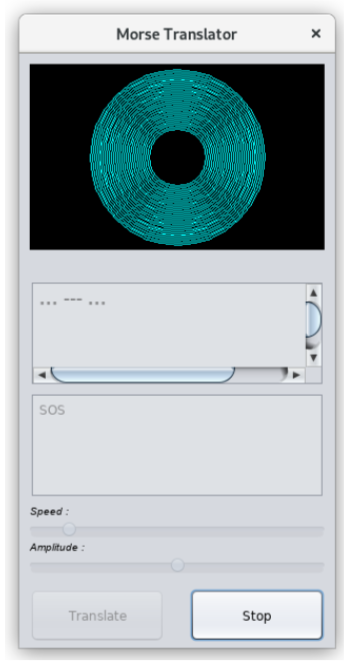
\includegraphics[scale=0.8]{descpicture.png}
    		\caption{Capture d'écran de l'application de test du composant}
    		\label{Capture d'écran de l'application de test du composant}
    	\end{center}
    \end{figure}
    
	\begin{figure}[H]
		\begin{center}
			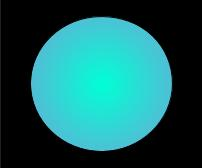
\includegraphics[scale=0.5]{comdescpicture.jpg}
			\caption{Interface graphique du composant}
			\label{Interface graphique du composant}
		\end{center}
	\end{figure}
    \subsection{Utilisation}
    

    \section{Model UML}
    \subsection{Diagramme d'état}
    \subsection{Diagramme des classes}
    \begin{figure}[H]
    	\parshape1 -4cm 21cm
    	\begin{center}
    		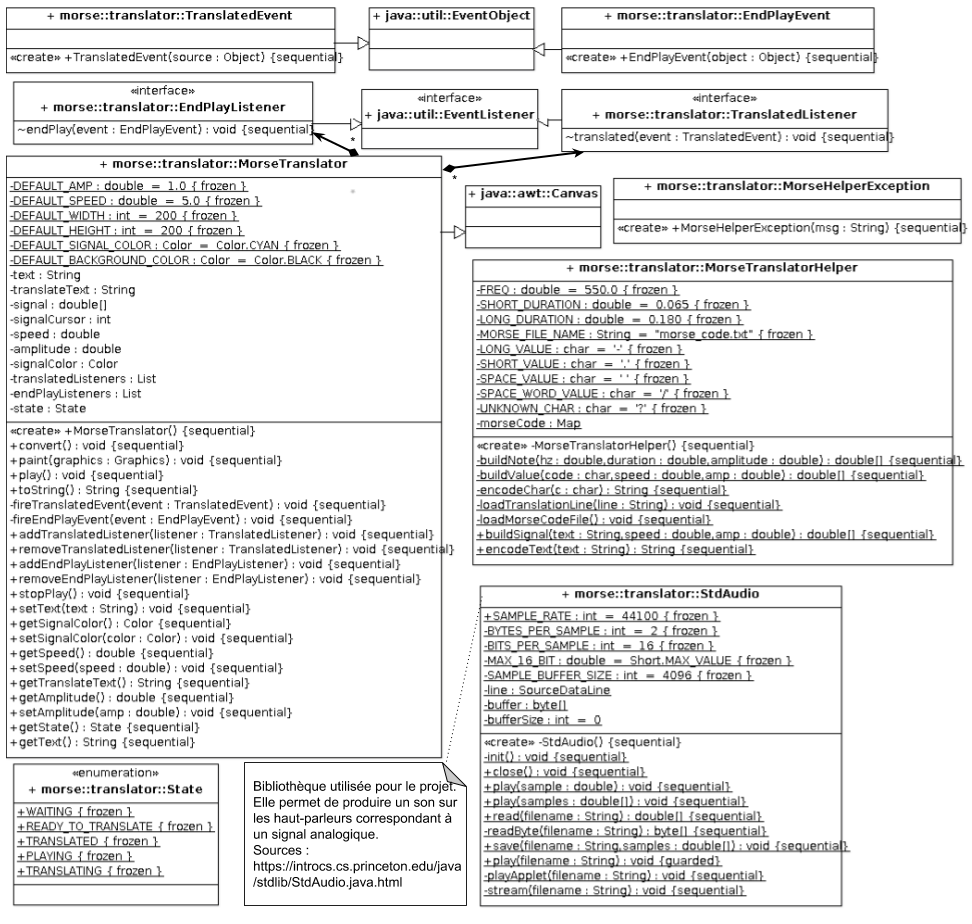
\includegraphics[scale=0.6]{classdiag.png}
    		\caption{Diagramme des classes UML}
    		\label{Diagramme des classes UML}
    	\end{center}
   		\parshape0
    \end{figure}

\end{document}
